\chapter{Analytical Model}
\label{ch:analyticalmodel}
\textit{This chapter intends to explain the calculation of the critical current in different SNS junctions. For this purpose, a quasiclassical transport theory is used and its foundations are explained in the first section. This technique is then employed for a clean SNS junction and an expression for the Josephson current is found. In the following section the calculations used for the clean setup are extended for the more sophisticated quantum point contact (QPC) and here as well, the current for the QPC-gated junction is found.}

\section{Foundation of the quasiclassical model}
\begin{figure}
\centering	
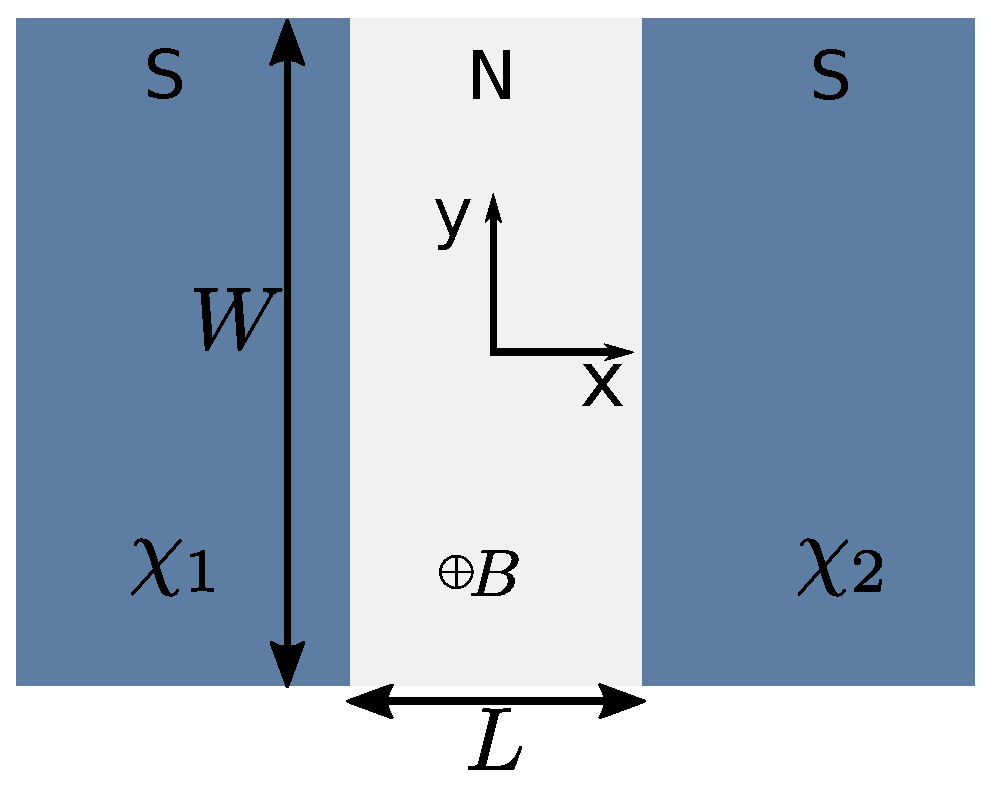
\includegraphics[width=0.6\textwidth]{figure/analyticalmodel/sns_junction}
\caption{Schematic representation of a short and wide SNS junction.}
\label{fig:sns_schematic}
\end{figure}
This section explains preliminary assumptions made to model the current in a SNS junction, a scheme of which is  shown in fig \ref{fig:sns_schematic}. The setup is two dimensional with width $W$ and length $L$ and a short and wide junction with $W \gg L$ is considered. The NS-interfaces are parallel to the $y$-axis and are placed at $x = \pm L/2$. Each of the superconducting leads has a phase $\chi_{1}$ and $\chi_{2}$ and the overall phase difference is $\chi = \chi_{1} - \chi_{2}$. The superconducting gap parameter is only present in the superconducting leads and zero in the normal region and can be expressed as
\begin{equation}
\Delta\left( x \right) = |\Delta| e^{\chi_1} \Theta\left(-L/2 -x \right) + |\Delta| e^{\chi_2} \Theta\left(x-L/2 \right) 
\label{eq:gap_parameter}
\end{equation}
The aim is to express the current through the junction using a quasiclassical approach. In this approach, the Andreev bound states are associated with straight trajectories connecting the superconducting leads. The superconducting current density is expressed in terms of these trajectories. We consider a ballistic sample with ballistic (BCS) coherence length $\zeta = \hbar v_F / \pi \Delta$ %TODO check!
We assume that at this coherence length $\zeta$ is much larger than the Fermi velocity $\zeta \gg v_F$ (in order to induce superconductivity in the system?). The relation between the coherence length $\zeta$ and the sample length $L$ determines, if the considered junction is a \textit{short} or a \textit{long} junction:
\begin{eqnarray*}
\zeta \ll L \quad \rightarrow \quad \text{long junction} \quad \rightarrow \quad \text{many Andreev levels} \\ 
\zeta \gg L \quad \rightarrow \quad \text{short junction} \quad \rightarrow \quad \text{one Andreev level} 
\end{eqnarray*}
Needless to mention, the fermi wavelength $\lambda_F$ has to be smaller than the sample length $L$. 
Now, check if this quasiclassical approach is valid. What are preliminary assumptions about the system?
%TODO klar machen, dass jetzt die Voraussetzungen für Modell getestet werden
The presence of magnetic field will lead to a bending of the trajectories due to the Lorentz force. Depending on the strength of magnetic field $B$ and the Fermi velocity the radius of this curve is 
\begin{equation}
r_B = ???
\end{equation}
%TODO add the formula for cyclotron radius
In order to justify the assumption of straight trajectories, either the magnetic field has to be weak enough or the Fermi wavelength has to be short enough. Then, the cyclotron radius $r_B$ is simply much smaller than the sample length $L$. 
We consider the low temperature limit, where the thermal length scale of the system is smaller larger than the sample length:
\begin{equation}
L_T = \hbar v_F / k_B T \gg L
\end{equation} 
%TODO what do these length scales mean? Add!

\section{Plane setup: calculation of current}
%TODO Re-calculate current from Glazman
To derive the current for the SNS setup depicted in figure \ref{fig:sns_schematic}, we start by writing down the Bogoliubov-de-Gennes-Hamiltonian for this system.
\begin{equation}
\begin{pmatrix}
-\frac{1}{2m} \nabla^2 - \epsilon_F & \Delta(x) \\
\Delta^*(x) & \frac{1}{2m} \nabla^2 + \epsilon_F 
\end{pmatrix}
\begin{pmatrix}
\psi_e \\
\psi_h
\end{pmatrix} = E 
\begin{pmatrix}
\psi_e\\
\psi_h
\end{pmatrix}
\end{equation}
The expression above uses eq. (\ref{eq:gap_parameter}) for the spatially dependent superconducting gap parameter $\Delta(x)$. This Schr\"odinger equation can be solved with boundary conditions at $x = \pm L/2$ and leads to the following wave functions:
\begin{equation}
\text{TODO: Insert equations!}
\end{equation}
%TODO calculate current and wavefunctionsx
\textbf{TODO: Hier fehlt die Herleitung f\"ur Wellenfunktionen, Ausdruck f\"ur den Strom etc.!}
Current density for short and long junction limit: 
In the short junction limit the current density can be derived from the scattering matrix formalism and it reads
\begin{equation}
\mathcal{J}^s (\chi) = \frac{\mathcal{T} \sin \chi}{\sqrt{1 - \mathcal{T} \sin^2 \frac{\chi}{2}}}
\end{equation}
$\mathcal{T}$ is the transmission coefficient that describes the transmission through a channel (each channel corresponds to a eigenvalue of the scattering matrix.
The current density for the long junction limit is
\begin{equation}
\mathcal{J}(\chi) = \sum_{k = 1}^{\infty} \frac{(-1)^{k+1}}{k} \sin( k \chi).
\end{equation}
\begin{figure}
\centering
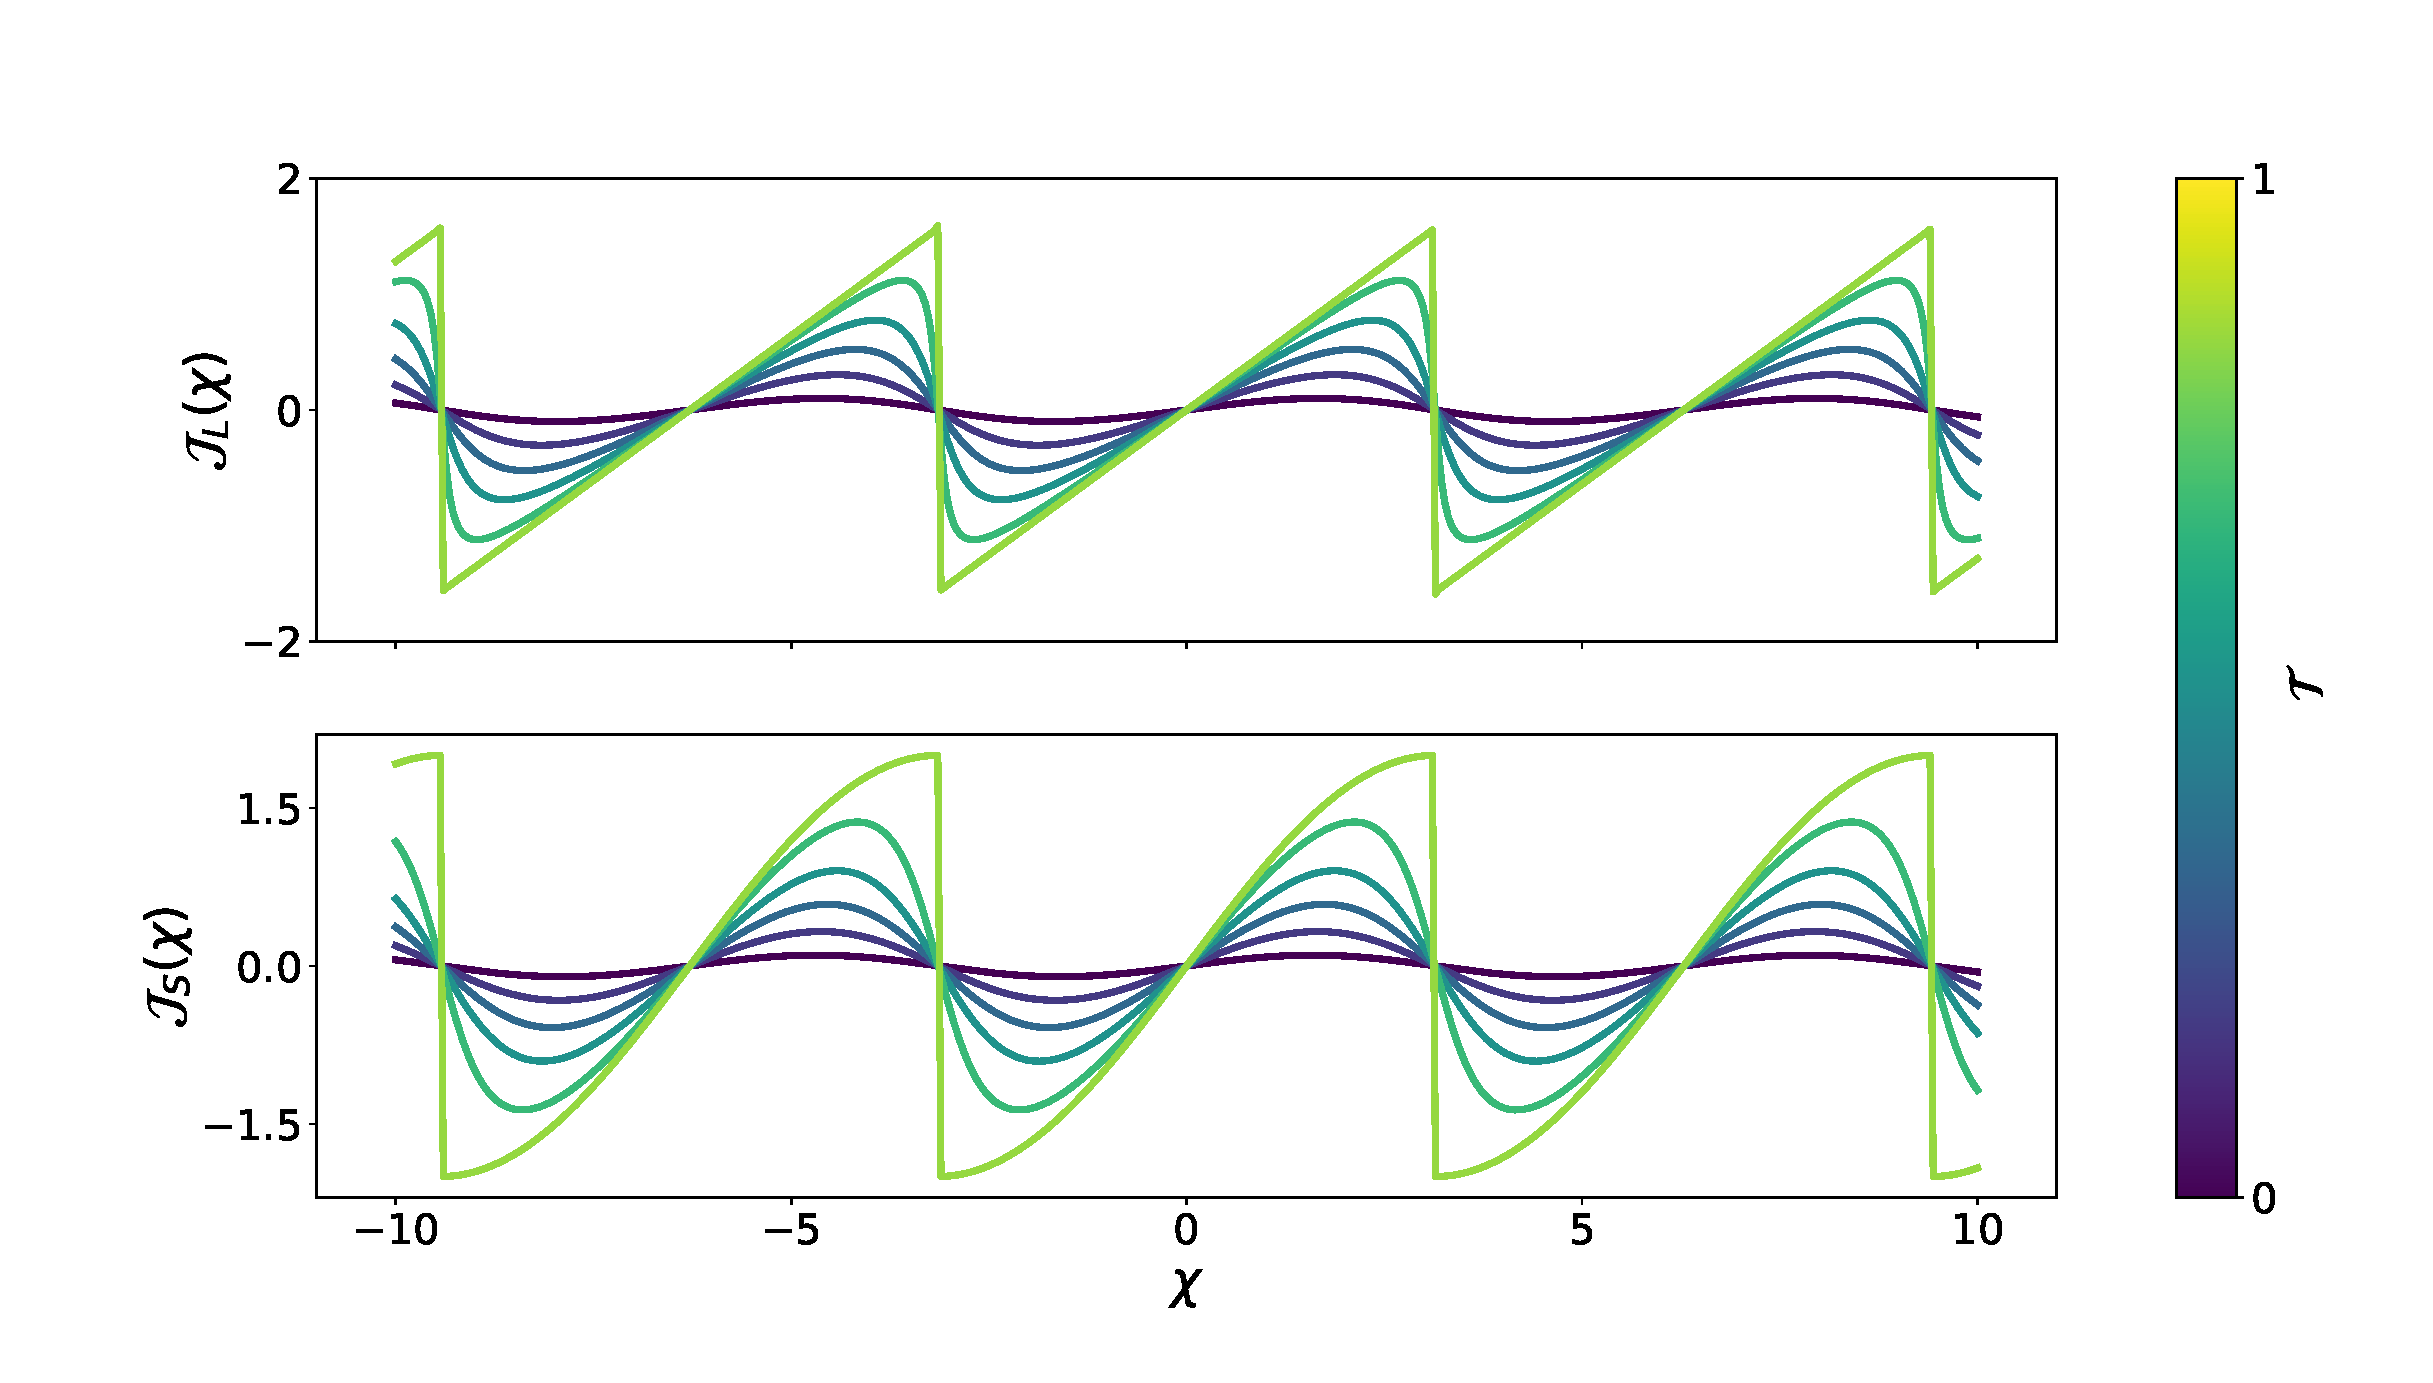
\includegraphics[width=\textwidth]{figure/analyticalmodel/current_density_all}
\caption{Short and long junction current density}
\label{fig:current_density}
\end{figure}
Figure \ref{fig:current_density} shows a plot of both short and long junction limit current densities. They differ for a large transmission coefficient $\mathcal{T} \simeq 1$, where in the long junction limit we observe a sawtooth like shape and in the short junction limit we have a sinusoidal shape.\\
Using the current density the Josephson current at zero magnetic field ($\phi = 0$) can be expressed as 
\begin{equation}
J\left(\chi, \phi=0\right) = \frac{2 e v_F}{\pi \lambda_F L^2}  \int \int_{-W/2}^{W/2} d y_1 d y_2 \frac{\mathcal{J}(\chi)}{\left[ 1 + \left(\frac{y_1 - y_2}{L}\right)^2\right]^2}
\label{eq:josephson_current_zero_b}
\end{equation}
\subsection*{Including magnetic field}
So far, the current has been derived for zero magnetic field. If a finite magnetic field is considered, the phase $\chi$ will be modified because of two effects. The magnetic phase that will be acquired along a trajectory connecting two points $y_1$ and $y_2$  leads to an additional term in the phase. Then again, \textit{the condition of zero screening current in the bulk superconducting region and the limit of} $\lambda_L \rightarrow 0$ \textit{require the superconducting phase at the interfaces to become functions of y} \textbf{TODO: ? Umschreiben!}.\\
Assuming that the London penetration depth is small to zero in the superconducting regions the following gauge for the vector potential can be used
\begin{equation}
\mathbf{A}=A_y \mathbf{e}_y, \quad
A_y=\left\{ 
		\begin{array}{ll}
				-B x, & -L/2 \leq x \leq L/2, \\[0.2cm] 
				-\frac{1}{2} B L |x| , & \quad |x|>L/2
		\end{array} 
	\right.
\label{eq:Ay}
\end{equation}
The gauge in eq. (\ref{eq:Ay}) will give no additional contribution to the phase on straight trajectories
\begin{eqnarray}
\delta \chi &=& \frac{2 \pi}{\Phi_0} \int d \mathbf{l} \cdot \mathbf{A} \\
&=& \frac{2 \pi}{\Phi_0} \int_{-L/2}^{L/2} \frac{dx}{\cos \theta} A_y (x) \sin \theta \\
&=& - \frac{2 \pi B}{\Phi_0} \frac{y_2 - y_1}{L} \int_{-L/2}^{L/2} x dx \\
&=& 0
\end{eqnarray}
and therefore, the only contribution to the magnetic phase is
\begin{equation}
\delta \chi = -\frac{\pi \phi (y_1 + y_2)}{W} \quad \Leftrightarrow \quad \tilde{\chi}(y_1, y_2) = \chi  -\frac{\pi \phi (y_1 + y_2)}{W}.
\label{eq:chi_plane}
\end{equation}
This mean that the current phase relation in the  expression for the Josephson current from eq. (\ref{eq:josephson_current_zero_b}) for zero magnetic field has to replaced by the effective phase $\chi \rightarrow \tilde{\chi}(y_1, y_2)$ and then reads
\begin{equation}
J\left(\chi, \phi \right) = \frac{2 e v_F}{\pi \lambda_F L^2}  \int \int_{-W/2}^{W/2} d y_1 d y_2 \frac{\mathcal{J}(\tilde{\chi}(y_1, y_2))}{\left[ 1 + \left(\frac{y_1 - y_2}{L}\right)^2\right]^2}
\label{eq:josephson_current}
\end{equation}
By maximizing the Josephson current with respect to $\chi$, the critical current can be found:
\begin{equation}
I_c(\phi) = \text{max}_{\chi}\left\{ J(\chi, \phi) \right\}
\end{equation}
\textbf{Dependence on W/L ratio? Further investigations? Plot of current?}

\section{Calculation of QPC current}
\begin{figure}
\centering
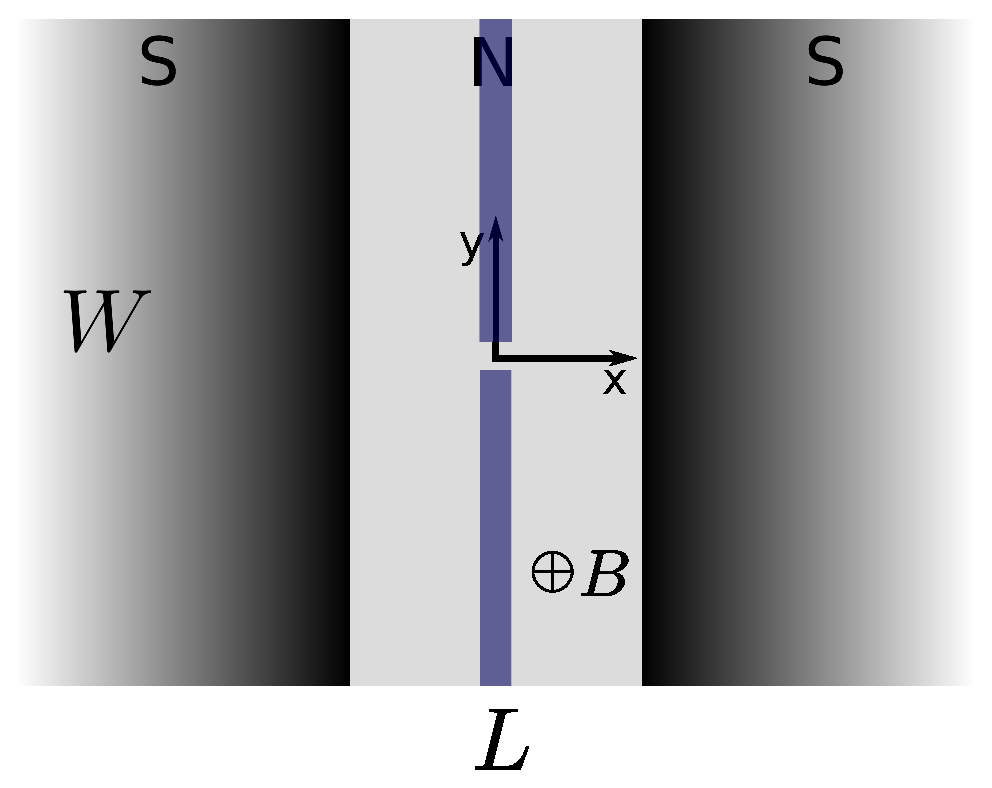
\includegraphics[width=0.6\textwidth]{figure/analyticalmodel/qpc_sns_junction}
\caption{QPC setup.}
\label{fig:qpc_sns_schematic}
\end{figure}
\textbf{TODO: what happens when a constriction is on top of normal layer, fermi levels etc}
The quasiclassical formalism can even be employed to modified SNS junctions. One can build gates on top of the normal region of the junction in a way that the current cannot pass through the gated regions. In the quasiclassical picture this means that the possibilites for trajectories connecting two points at the superconducting interfaces are limited through the geometry of the constriction.\\
Figure \ref{fig:qpc_sns_schematic} shows a schematic of the quantum point contact setup which will be analysed with the quasiclassical formalism. The normal region of the SNS junction is covered by a gate in the middle that has a small split in the middle. The split is located at $(x y) = (0, 0)$ so that the sample is symmetric around the origin. The width of the split is in the order of $\lambda_F$ (\textbf{Warum wichtig?}) and can thereby be modelled as an isotropic scattering point with transmission coefficient $\mathcal{T}_0$. Consequently, each trajectory connecting the two superconducting interfaces have to pass through the QPC. For simplicity the geometrical width of the barrier is neglected and only straight trajectories (no scattering at side edges) are considered. This modified setup leads first to a different parametrisation of the trajectories and therefore to a different magnetic phase than in eq. (\ref{eq:chi_plane}).\\
With the QPC setup, all possible trajectories are parametrised by two angles $\theta_i$ and $\theta_f$. $\theta_i$ describes the trajectory before passing through the QPC in the region $ -L/2 < x 0$ and  $\theta_f$ after passing through the QPC. The parametrisation of the trajectories reads
\begin{equation}
\tan \theta_i = - \frac{2 y_i}{L}, \quad \tan \theta_f = \frac{2 y_f}{L}
\end{equation}
With the gauge from eq. (\ref{eq:Ay}) the magnetic phase acquired within the sample reads:
\begin{eqnarray}
\frac{2\pi}{\Phi_0} \int d\mathbf{l} \cdot \mathbf{A}  &=&
-\frac{\pi B}{\Phi_0}\left(\frac{L}{2}\right)^2
\left(-\tan\theta_i + \tan\theta_f\right) =
-\frac{\pi \phi (y_i+y_f)}{2 W}.
\label{eq:phaseQPC}
\end{eqnarray}
Therefore the effective phase is
\begin{equation}
\tilde{\chi}(y_i,y_f)=\chi-\frac{3\pi \phi }{2W}(y_i+y_f).
\label{eq:chiQPC}
\end{equation}
The effective phase for the QPC in eq. (\ref{eq:chiQPC}) is half of to the effective phase without any constriction, in eq. (\ref{eq:chi_plane}). This seems reasonable, since in the QPC setup the all possible straigth trajectories can cover only half of the normal region compared to the setup without constriction.
The effective phase therefore modifies the current phase relation $\mathcal{J}(\tilde{chi}(y_i, y_f)$. Beyond that, the expression for the critical current has to be modified as well.

The normalized critical current reads
\begin{eqnarray}
\frac{I_c(\phi)}{I_c(0)} &=& \frac{ \text{max}_{\chi} \int d \theta_i \cos^2 \theta_i\int d \theta_f \cos \theta_f \mathcal{J}(\tilde{\chi}(\theta_i, \theta_f)) }{ \text{max}_{\chi} \int d \theta_i \cos^2 \theta_i\int d \theta_f \cos \theta_f \mathcal{J}(\chi) }
\end{eqnarray}
In the limit of small transmission probability $\mathcal{T} << 1$ we use Eq.~(\ref{sawT<1}) for the partial Josephson current. The normalized critical current can then be written as 
\begin{eqnarray}
\frac{I_c(\phi)}{I_c(0)} &=& \frac{\mathcal{I}_2(\phi)\mathcal{I}_{3/2}(\phi)}{\mathcal{I}_2(0)\mathcal{I}_{3/2}(0)}
\end{eqnarray}
Here, the integrals $\mathcal{I}$ are defined as
\begin{equation}
\mathcal{I}_k(\phi) = \frac{2}{L}\int_{-W/2}^{+W/2}dy \frac{\cos\left(\frac{3\pi\phi y}{2W}\right)}{\left[1 + \left(\frac{2y}{L}\right)^2 \right]^k}
\label{integral-qpc}
\end{equation}
At $\phi=0$ we get
\begin{equation}
\mathcal{I}_2(0)\mathcal{I}_{3/2}(0) =
\frac{L}{\sqrt{L^2+W^2}}\arctan\frac{W}{L} + \frac{L^2W}{(L^2+W^2)^{3/2}}
\label{Ic-0}
\end{equation}
The parabolic asymptotics of the critical current at small $\phi$ is found by expanding
the cosine factors in the numerator:
\begin{eqnarray}
\frac{I_c(\phi)}{I_{c0}}&\simeq& 1 - \frac{9\pi ^2 \phi^2 }{32} f_0(W/L) \\
f_0(x) &=& \frac{\sqrt{x^2+1} \log \left(\sqrt{x^2+1}+x\right)}{x}- \frac{x}{x+\left(x^2+1\right) \arctan(x)} 
\end{eqnarray}
In the opposite limit of high fields, $\phi\to \infty$, we extend the integration in Eq.~(\ref{integral-qpc}) over $y_i$ and $y_f$ to $\pm \infty$ and obtain
\begin{eqnarray}
\frac{I_c(\phi)}{I_{c0}} &\simeq& \frac{\pi^3 }{8x^2}\left(\frac{3\phi}{2x}\right)^{3/2}\frac{\left(1+x^2\right)^{3/2}}{x + \left(1+x^2\right)\arctan x}\exp\left(-\frac{3\phi\pi}{2x}\right)
\label{large-phi}
\end{eqnarray}
change in magnetic phase, geometrical argument, change in current, limits etc. 

%TODO wie weiter?
%Skizze erklären, wie ist das QPC aufgebaut?
%Was ändert sich für den Strom? 
%Wie sieht das Ergebnis aus?



